

Sedaj predstavljena metoda empirične primerjave, se lahko uporabi za empirično primerjavo med priponskimi drevesi in kompaktnimi priponskimi drevesi. Primerjava je bila izdelana s programskim jezikom C++ \footnote{Koda je dostopna na povezavi \url{https://github.com/GioGiou/MagisterskaNalogaKoda}.}. Priponska drevesa so bila izgrajena z Ukkonenovim algoritmom implementiran v C++ knjižnici \cite{ganeshk13}. Kompaktna priponska drevesa so bila izgrajena s predhodno predstavljeno metodo. Uporabljena je bila implementacija kompaktnih priponskih dreves iz C++ knjižnice \cite{gbmp2014sea}.

Evalvacija je bila izvedena na računalniku s procesorjem Intel Core i3 5005U z dvema jedroma in štirimi nitmi ter s taktom 1,9 GHz. Računalnik ima na razpolago 4 GB delovnega spomina, od katerega je ob zagonu računalnika zasedenih 1,76 GB, ter ima še dodatnih 8 GB \verb|Swap| razdelka na trdem disku. Operacijski sistem računalnika je Fedora 41, ki uporablja Linux kernel 6.11.10-300. 

Ob testiranju izgradnje večjih priponskih dreves je bilo opaženo, da operacijski sistem ubije (angl. \textit{kill}) proces, ki izvaja testiranje, zaradi nevarnosti o preseganja velikosti delovnega spomina. To se je zgodilo pri izgradnji priponskega drevesa velikosti 4000000 znakov. Pri tem se je tudi opazilo, da pri priponskem drevesu velikosti 2048000 znakov ni mogoče izgraditi drevesa do konca, saj računalnik ne uspe premakniti strani iz delavnega pomnilnika na \verb|Swap| razdelek in obratno. To naredi računalnik  neodziven in proces je v neprekinjenem spanju (angl. \textit{Uninterruptible sleep} ali stanje D), pri tem računalnik doseže 6 GB zasedenega prostora na \verb|Swap| razdelku. Na Sliki \ref{fig:6GB} je prikazan upravljalnik opravil Htop v času izgradnje priponskega drevesa za  besedilo velikosti 2048000 znakov. Proces v modri vrstici predstavlja program za testiranje izgradnje besedil. V stolpcu označenim S (Stanje ali angl. \textit{Status}) je vidno, da je je stanje procesa označeno kot D, ker je proces v neprekinjenem spanju. Po več kot 5 minutah od začetka izgradnje prvega priponskega drevesa sem se odločil, da se proces ubije. Posledično se je znižala velikost besedil za izgradnjo zadnjega priponskega drevesa na 1024000 znakov.

\begin{figure}[tb]
    \centering
    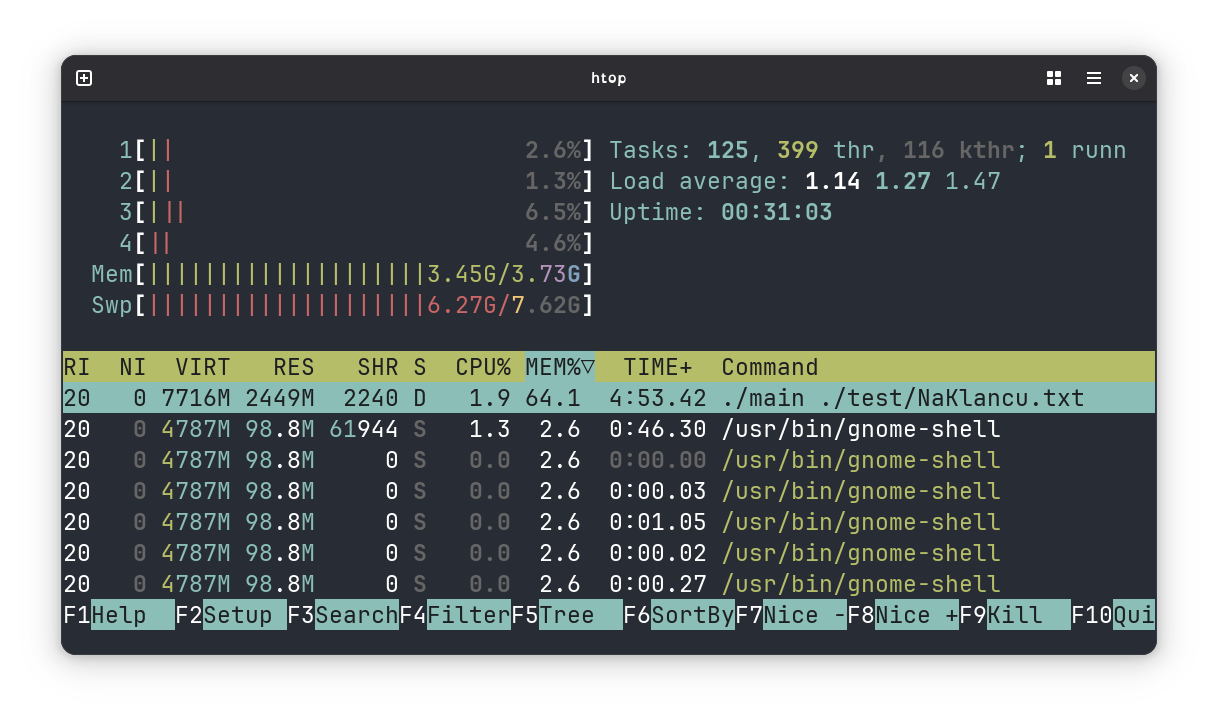
\includegraphics[width=\textwidth]{Slike/Zaslonski posnetek 2025-06-23 22-53-56.png}

    \captionof{figure}[Posnetek zaslona upravljalnika opravil Htop med izgradnjo priponskega drevesa za besedilo dolžine 2048000 znakov.]{Posnetek zaslona upravljalnika opravil Htop med izgradnjo priponskega drevesa za besedilo dolžine 2048000 znakov.} 
    \label{fig:6GB}
\end{figure}

\newpage
Pri tem se je tudi omejila velikost besedila $B_0$ na $S_{max}=25000000$ znakov. To zagotavlja dovolj znakov za izgradnjo vhodnih besedil ter za izgradnjo besedil, ki bodo predstavljali vzorce. Ker je DNK sekvenca \cite{podatki} daljša od velikosti $S_{max}$, je bila le ta odrezana na velikost $S_{max}$ in sicer bo uporabljeni le prvih 25000000 znakov. Za razliko od DNK sekvence, je besedilo Na klancu \cite{podatkiNaKlancu} moralo biti podaljšano na $S_{max}=25000000$ znakov. To je bilo storjeno z implementacijo Algoritma \ref{alg:Konkatenacija} v programskem jeziku C++. Pri tem ni bilo potrebno implementirati preverjanja, ali šestkratnik števca $i$ presega velikost besedila $B$. Torej tega nisem storil.

Čas potreben za izgradnjo priponskega drevesa in izvršitev poizvedb je bil izmerjen s pomočjo razlike v uri pred in po izvršitvi testa, kot je to bilo predhodno opisano. Meritev je bila implementirana s funkcijo \verb|high_resolution_clock::now()|, ki je del standardne knjižnice programskega jezika C++ in vrne natančen čas trenutka, v katerem je izvedena.
S tako izmerjenim časom pred začetkom in takoj po koncu izvajanja se lahko naračuna razliko s funkcijo \verb|duration_cast<milliseconds>(stop - start).count()|, kjer \verb|stop| predstavlja čas konca izvajanja in \verb|start| pa predstavlja čas začetka izvajanja operacije. Funkcija vrne v tem primeru razliko med tema dvema trenutkoma v milisekundah, ki pa se lahko po potrebi zamenja v druge časovne enote. V primeru poizvedb je bil čas iskanja vzorca izmerjen v nanosekundah in je bil implementiran s pomočjo funkcije \verb|duration_cast<nanoseconds>(stop - start).count()|.

Vektorja rezultatov testiranja $T_{i,v}$ in $S_{i,v}$ sta bila zapisana v CSV (angl. \textit{Comma-separated values}) datoteko za lažjo nadaljnjo obdelavo rezultatov. Vsaka vrstica datoteke predstavlja rezultat enega testiranja. Poleg vektorjev  $T_{i,v}$ in $S_{i,v}$, je v vsaki vrstici zapisana velikost začetnega besedila $i$ ter vrsta priponskega drevesa $v$. Ker se med izvajanjem programa ne beleži velikost priponskega drevesa, se zato zapiše začasna vrednost.

Predhodno predstavljena implementacija je bila izdelana v datoteki \verb|main.cpp|. Koda je bila prevedena iz programskega jezika C++ v izvršljivo datoteko z uporabo prevajalnika (angl. \textit{compiler}) GCC 14.2.1. Program je bil preveden s sledečim ukazom:
\begin{lstlisting}[language=bash]
    g++ -std=c++11 -O3 -DNDEBUG -I ./include -L ./lib // 
    main.cpp -o main -lsdsl -ldivsufsort //
    -ldivsufsort64 -lsuffix
\end{lstlisting}
Pri prevajanju programa je uporabljenih nekaj zastavic, ki določajo vrednosti parametrov prevajalnika. Večina zastavic je vezana na uvažanje knjižnic v prevajanje, in sicer \verb|-I ./include| nastavi pot do zaglavnih datotek (angl. \textit{header files}), \verb|-L ./lib| nastavi pot do strojne kode knjižnice ter zastavice \verb|-lsdsl|, \verb|-ldivsufsort|, \verb|-ldivsufsort64| in \verb|-lsuffix| uvozijo potrebne knjižnice za izgradnjo izvršljive datoteke.
Zastavica \verb|-O3| določa nivo optimizacije izvršljive datoteke, na nivo 3, ki je bil izbran, saj je uporabljen za prevajanje prve implementacije kompaktnega priponskega drevesa \cite{Valimaki2007}.
%Zastavica \verb|-DNDEBUG| ne preverja pravilnosti vseh trditev, kar zniža velikost izvršljive datoteke.
Pri izgradnji programa je bila uporabljena standardna različica C++11 določena z zastavico \verb|-std=c++11|. Razlog za izbiro starejše različice programskega jezika je knjižnica SDSL \cite{gbmp2014sea} (uporabljena kot implementacija kompaktnih priponskih dreves), ki je implementirana za to različico. 

Ker tako prevedena datoteka ne omogoča neposrednega nadzorovanja velikosti podatkovnih struktur med izvajanjem, bo za ta namen uporabljen profiler spomina. Zato je potrebo pred začetkom testiranja priponskih dreves zagnati tudi profiler, kar je storjeno z ukazom:
\begin{lstlisting}[language=bash]
    export MEMORY_PROFILER_LOG=info
    LD_PRELOAD=~/bytehound/libbytehound.so ./main // 
    ./test/NaKlancu.txt 
\end{lstlisting}
Prva vrstica ukaza določa stopnjo profiliranja, ki ima v tem primeru vrednost \verb|info|, ter jo shrani v sistemsko spremenljivko \verb|MEMORY_PROFILER_LOG|. Naslednja vrstica pa požene program na datoteki s testnimi podatki, ki so podani kot prvi argument (ime datoteke). Zgornji ukaz prikaže primer za vhodno besedilo Na klancu. S spremenljivko \verb|LD_PRELOAD| je določen deljeni objekt (angl. \textit{shared object}), ki je izvršen pred začetkom programa. V primeru testiranja priponskih dreves je deljeni objekt profiler, kar mu omogoča dostop do programa in lažje beleženje zasedenega delovnega spomina.

\newpage
Prva izdelana primerjava priponskega drevesa in kompaktnega priponskega drevesa je izdelana nad 50 MB dolgo DNK sekvenco \cite{podatki}. Kot vsa ostala testna besedila, je tudi DNK sekvenca shranjena v mapi \verb|./test/| pod imenom \verb|DNA.50MB|. Izbrana je bila, saj so jo uporabili kot testno besedilo v implementaciji od Välimäki idr. \cite{Valimaki2007}. Sekvenca je zlepek različnih DNK sekvenc.

Kot je bilo predstavljeno v Tabeli \ref{tab:besedila} je besedilo sestavljeno iz $4+1$ znakov. Izmerjen je bil tudi potreben prostor za shranjevanje vhodnega besedila, ki zasede $26,767$ MB delovnega spomina. Velikost zasedenega prostora na delovnem spominu z vhodnim besedilom je potrebno odšteti od velikosti, ki jo potrebujejo implementirana priponska drevesa.

\begin{figure}[htb]
    \centering
    \includesvg[inkscapelatex=false,width=\textwidth]{Slike/velikostDrecvesaNovPC.svg}
    \captionof{figure}[Graf velikosti priponskega drevesa izgrajenih iz besedil različne velikosti. Vhodno besedilo je DNK sekvenca.]{Graf velikosti priponskega drevesa izgrajenih iz besedil različne velikosti. Vhodno besedilo je DNK sekvenca.} 
    \label{fig:VelikostGraf}
\end{figure}

Na Sliki \ref{fig:VelikostGraf} je prikazana potrebna količina delovnega spomina za izgradnjo priponskega drevesa, ki je označena z modro, ter kompaktnega priponskega drevesa, ki pa je označena z rdečo barvo. Na sliki je uporabljena, na vodoravni osi, logaritmična skala za velikost besedila, saj je vsako naslednje testirano besedilo dvakrat večje od predhodnega. Iz slike se lahko jasno vidi, da za besedila do dolžine 8000 znakov obe drevesi zasedeta približno enako količino prostora na delovnem spominu, in sicer priponsko drevo zasede $39,8$ MB in kompaktno priponsko drevo zasede $27,4$ MB. Vse nadaljnje razlike v velikosti med priponskim drevesom in kompaktnim priponskim drevesom so izrazite. Čeprav se zdi, da je velikost kompaktnega priponskega drevesa konstanta, se ta v času izvajana testiranja dvigne iz približno $27,4$ MB na približno $29$ MB.

Na Sliki \ref{fig:VelikostGraf} se lahko tudi opazi, da velikost priponskega drevesa ne presega $4$ GB, kar je velikost notranjega spomina. Pri tem pa je potrebno upoštevati dejstvo, da operacijski sistem potrebuje $1,76$ GB delovnega spomina takoj po zagonu računalnika. To pomeni, da čeprav velikost priponskega drevesa ne presega velikosti delovnega pomnilnika, mora biti le ta shranjen v \verb|Swap| razdelku, saj mora računalnik v vsakem trenutku zagotoviti dovolj prostora na delovnem pomnilniku za operacijski sistem, torej ima program na razpolago največ $2,24$ GB delovnega pomnilnika. Zadnje testirano priponsko drevo potrebuje $3,56$ GB dolgovnega pomnilnika, zato mora biti vsaj $1,22$ GB drevesa shranjenega v na \verb|Swap| razdelku.

\begin{figure}[htb]
    \centering
    \includesvg[inkscapelatex=false,width=\textwidth]{Slike/izgradnjaDrecvesaNovPC.svg}
    \captionof{figure}[Graf prikazuje čas izgradnje priponskega drevesa za različne dolžine vhodnih besedil. Vhodno besedilo je DNK sekvenca.]{Graf prikazuje čas izgradnje priponskega drevesa za različne dolžine vhodnih besedil. Vhodno besedilo je DNK sekvenca.} 
    \label{fig:IzgradnjaGraf}
\end{figure}

Ker je zadnje izgrajeno priponsko drevo, moralo biti shranjeno tudi na \verb|Swap| razdelku, je potrebno preveriti, na kakšen način to vpliva na čas izgradnje drevesa ter iskanje v njem. Rezultati testiranja časa izgradnje različnih implementacij priponskega drevesa so prikazani na Sliki \ref{fig:IzgradnjaGraf}, kjer z modro barvo je prikazan čas potreben za izgradnjo priponskega drevesa ter z rdečo pa čas potreben za izgradnjo kompaktnega priponskega drevesa. Vsi časi, ki so prikazani na sliki, so v milisekundah.

\newpage
Pri izgradnji največjega priponskega drevesa se lahko opazi na Sliki \ref{fig:IzgradnjaGraf}, da je potrebni čas višji od pričakovanega. Skok v časovni zahtevnosti se pojavi, pri izgradnji priponskega drevesa, ki je moral biti delno shranjen na \verb|Swap| razdelku. Vsa ostala priponska drevesa so zgrajena dvakrat počasneje kot predhoden priponsko drevo, kar je tudi pričakovano, saj Ukkonenov algoritem izgradi priponsko drevo v času $O(n)$. Torej, ker se je velikost besedila podvojila, potemtakem se bo tudi čas izgradnje podvojil. Izjema je zadnje izgrajeno priponsko drevo (dolžina vhodnega besedila je 1024000 znakov), kjer se čas izgradnje poveča za $4,78$-krat. Iz tega se lahko sklepa, da uporaba \verb|Swap| razdelka negativno vpliva na čas izgradnje priponskega drevesa.

Iz Slike \ref{fig:IzgradnjaGraf} je tudi razvidno, da čas potreben za izgradnjo kompaktnega priponskega drevesa raste počasneje kot čas izgradnje priponskega drevesa. Čas potreben za izgradnjo kompaktnega priponskega drevesa za besedilo dolžine 500 znakov je $70,8$ milisekund, čas za izgradnjo kompaktnega priponskega drevesa za besedilo dolžine 1024000 znakov pa je $121$ milisekund. Kompaktno priponsko drevo se zgradi hitreje od priponskega drevesa pri besedilih, ki so daljši od 8000 znakov. Priponsko drevo potrebuje $83,2$ milisekunde za izgradnjo, za razliko od kompaktnega priponskega drevesa, ki pa potrebuje $75,2$ milisekunde za biti izgrajeno nad besedilom dolžine 8000 znakov.

\begin{figure}[htb]
    \includesvg[inkscapelatex=false,width=\textwidth]{Slike/IskanjeNovPC.svg}
    \captionof{figure}[Graf prikazuje čas iskanja vzorcev različnih dolžin v različnih implementacijah priponskega drevesa. Vhodno besedilo je DNK sekvenca.]{Graf prikazuje čas iskanja vzorcev različnih dolžin v različnih implementacijah priponskega drevesa. Vhodno besedilo je DNK sekvenca.} 
    \label{fig:IskanjeGraf}
\end{figure}

Nazadnje se lahko še analizira vpliv velikosti priponskega drevesa na potreben čas za izvršiti poizvedb nad njim. Na Sliki \ref{fig:IskanjeGraf} so prikazani časi, v nanosekundah, potrebni za iskanje vzorcev, in sicer z modro barvo so predstavljeni časi za poizvedbe v priponskih drevesih, z rdečo pa so predstavljeni časi za poizvedbe v kompaktnem priponskem drevesu. Na sliki so predstavljeni rezultati za vse štiri velikosti vzorcev iskanih v priponskem drevesu: 5 znakov, 50 znakov, 500 znakov in $\log{n}$ znakov, pri čemer je $n$ dolžina besedila.

Na Sliki \ref{fig:IskanjeGraf} so prikazani rezultati primerjave iskanja vzorcev dolžine 5 znakov. Časi potrebni za iskanje vzorca so za obe implementaciji priponskih dreves podobni in konstantni. Edina vidna razlika je v času, ki je potrebnem za najdi vzorec v priponskem drevesu dolžine 1024000 znakov. To je posledica uporabe \verb|Swap| razdelka, zato se potrebuje $7,46$-krat več čas od ostalih poizvedb s priponskim drevesom. Ostale poizvedbe, za vzorce dolžine 5 znakov, potrebujejo približno 1000 mikrosekund, pri čemer pa priponsko drevo za besedilo dolžine 1024000 znakov pa potrebuje $8,79$ milisekund za preveriti prisotnost vzorca. Čas, ki je potreben za poizvedbo v kompaktnih priponskih drevesih, je konstanten in je približno $3,2$ mikrosekunde.

Za vzorce dolžine 50 znakov je iz Slike \ref{fig:IskanjeGraf} razvidno, da so potrebni časi za iskanje podobni kot pri iskanju vzorcev dolžine 5 znakov. Torej je čas, ki je potreben za iskanje v priponskem drevesu, konstanten in je  približno $2,2$ mikrosekunde. Ko priponsko drevo preraste delovni spomin in mora bit delno shranjen na \verb|Swap| razdelku se iskalni čas poveča za  $7,44$-krat. Pri tem iskanje vzorcev dolžine 50 znakov potrebuje približno enako časa kot iskanje vzorcev v kompaktnem priponskem drevesu. V kompaktnem priponskem drevesu je potrebnih približno $1,5$ mikrosekunde za preveriti ali je vzorec prisoten ali ni. Iz tega se lahko sklepa, da za iskanje vzorcev dolžine 50 znakov je bolj učinkovita uporaba priponskih dreves za besedila do 8000 znakov, ko je potrebno tudi izgraditi priponsko drevo. Za besedila daljša od 8000 znakov pa je bolje uporabiti kompaktno priponsko drevo.

Iskanje prisotnosti vzorca dolžine 500 znakov, rezultati so prikazani na Sliki \ref{fig:IskanjeGraf} kot predzadnji graf, je bolj učinkovito s priponskimi drevesi. Čeprav je za vse testirane velikosti priponskega drevesa iskanje v priponskem drevesu hitrejše ali primerljivo z iskanjem v kompaktnem priponskem drevesu, se lahko opazi rast v potrebnem času v večjih priponskih drevesih, ki so deloma shranjena v \verb|Swap| razdelku. Čeprav razlika ni tako očitna kot v primeru iskanja vzorca dolžine 5 ali 50 znakov, se lahko vseeno vidi rast iz grafa. Možen razlog za nižjo rast je prisotnost strani (angl. \textit{page}), ki vsebujejo vzorec v delovnem spominu in ne na \verb|Swap| razdelku. Pri tem je vseeno potrebna $1$ mikrosekunda za najti vzorec dolžine 500 znakov. Čas iskanja vzorcev v kompaktnih priponskih drevesih še vedno ostane konstantno, pri čemer se potreben čas za iskanje vzorcev dolžine 500 znakov zniža na $1,5$ mikrosekunde. Iz testiranja iskanja vzorcev velikosti 500 znakov v priponskih dresih se lahko sklepa, da če je na razpolago dovolj prostora na delovnem spominu, je boljše uporabiti priponsko drevo za te namene.

Zadnje testiranje, ki je prikazano na Sliki \ref{fig:IskanjeGraf}, je iskanje vzorcev dolžine $O(\log(n)$, pri čemer je $n$ velikost besedila, ki je predstavljeno s priponskim drevesom. Velikosti iskanih vzorcev se gibajo od 9 znakov do 20 znakov. Iz grafa je razvidno, da kompaktno priponsko drevo, označeno na grafu z rdečo barvo, potrebuje približno konstanto časa za najti vzorec v priponskem drevesu. Za iskanje vzorca potrebuje približno $4,5$ mikrosekunde. Pri tem pa je zgodba bistveno drugačna pri iskanju vzorcev s pomočjo priponskega drevesa, ki je prikazano z modro barvo na sliki. Za vzorce velikosti 9 in 10 znakov je čas iskanja v priponskem drevesu višji kot čas iskanja v kompaktnem priponskem drevesu. V vseh ostalih primerih pa je čas iskanja nižji kot v kompaktnem priponskem drevesu, podobno kot pri iskanju vzorcev dolžine 500 znakov. Iskanje vzorca dolžine 11 znakov ali več potrebuje približno $1$ mikrosekundo, da se izvrši. Pri tem se lahko tudi opazi, da je čas iskanja v zadnjem drevesu $4,5$-krat višji zaradi uporabe \verb|Swap| razdelka, kar pomeni, da potrebuje približno enako časa kot iskanje v ekvivalentnem kompaktnem priponskem drevesu. Iz tega testa se lahko sklepa, da za iskanje krajših vzorcev (vzorci do dolžine 10 znakov) je boljše uporabiti kompaktno priponsko drevo, sicer pa je boljše uporabiti priponsko drevo, če velikost delovnega spomina to omogoča ter če je število iskanih vzorcev dovolj veliko. S tem se lahko amortizira čas iskanja vzorcev, pri čemer je število vzorcev $O(n)$, kar zniža čas izgradnje drevesa za vsak vzorec na $O(1)$.

Iz testiranja izgradnje priponskega drevesa ter izvajanje poizvedb nad njim, za DNK sekvence je za iskanje v besedilih velikost do 8000 znakov boljše uporabiti priponsko drevo. Uporaba priponskega drevesa je tudi priporočljiva za daljše vzorce, kot so na primer vzorci dolžine 500 znakov. Pri tem mora biti število iskanih vzorcev dovolj veliko, da se amortizira čas, ki je potreben za izgradnjo priponskega drevesa (število vzorcev je $O(n)$), sicer je za vsako priponsko drevo zgrajeno nad besedilom z vsaj 8000 znaki bolj priporočljivo, da se za iskanje uporablja kompaktno priponsko drevo. Uporaba kompaktnih priponskih dreves se izkaže boljša pri iskanju krajših vzorcev ter ko velikost priponskega drevesa presega velikost notranjega pomnilnika in zato mora bit shranjeno delno ali v celoti na \verb|Swap| razdelku.

Druga primerjava je bila narejena s Cankarjevim romanom Na klancu \cite{podatkiNaKlancu}. Namen te primerjave je primerjati lastnosti priponskega drevesa nad večjo začetno abecedo, kot je na primer abeceda naravnega jezika. Ker slovenščina uporablja ne ASCII znake, je potrebno pred samim začetkom testiranja besedilo pred pripraviti. To je bilo storjeno tako, da so bili vsi ne ASCII znaki odstranjeni oziroma zamenjani z ASCII alternativami. Na primer znak, ki predstavlja '...', je bil zamenjan s tremi pikami, vse črke z naglasi (kot so strešice, ostrivci ter drugi) so bile zamenjani z osnovnim znakom, torej na primer š postane s in é postane e. Pri tem so bile tudi odstranjene vse prazne vrstice ter ločila poglavij, ki so bila označena z '***'. Odstranjeni so bili tudi vsi nevidni simboli, ki niso videni bralcu, prisotni v besedilu. Na ta način se je začetno besedilo znižalo iz dolžine 319843 znakov na 317803 znakov pred podaljševanjem. Naslednji korak je bila podaljšava besedila, ki podaljša velikost besedila iz 317803 na 25000000 znakov.

Uporabljeno besedilo uporablja abecedo velikosti $52+1$ znak, pri čemer je originalna abeceda sestavljena iz slovenske abecede brez črk 'č', 'š', in 'ž' (bodisi v velikih črkah bodisi v malih črkah), ločil, presledkov in narekovajev. Pri tem vhodno besedilo zasede $25,851$ MB delovnega spomina, kar je všteto v vse meritve velikosti različnih implementacij priponskih dreves.

\begin{figure}[htb]
    \includesvg[inkscapelatex=false,width=\textwidth]{Slike/velikostDrecvesaNovPCSLO.svg}
    \captionof{figure}[Graf velikosti priponskega drevesa izgrajenih iz besedil različnih velikosti. Vhodno besedilo je roman Na klancu.]{Graf velikosti priponskega drevesa izgrajenih iz besedil različnih velikosti. Vhodno besedilo je roman Na klancu.} 
    \label{fig:VelikostGrafSLO}
\end{figure}

Podobno kot za DNK sekvenco je bila izmerjena velikost, ki je potrebna za priponsko drevo na delavnem spominu. Rezultati meritve so prikazani na Sliki \ref{fig:VelikostGrafSLO}, kjer je z modro barvo prikazana velikost priponskega drevesa z rdečo barvo pa velikost kompaktnega priponskega drevesa. Za to besedilo je velikost prionskega drevesa manjša ali približno enaka (manj kot $1,5$-krat večja od kompaktnega prionskega drevesa) kompaktnemu priponskemu drevesu, do besedila dolžine 4000 znakov. Velikosti priponskih dreves rastejo dokler ne dosežejo velikosti $3,9$ GB za besedilo dolžine 1024000 znakov. Čeprav ima priponsko drevo velikost delovnega pomnilnika, mora biti skoraj polovica drevesa shranjena na \verb|Swap| razdelku, saj operacijski sistem zasede $1,76$ GB delovnega spomina. Pri tem se zdi, kot da kompaktno priponsko drevo ohranja konstantno velikost v vsakem testiranju. To se zgolj zdi, saj kompaktno priponsko drevo potrebuje bistveno manj prostora kot največje testirano priponsko drevo. Velikost kompaktnega priponskega drevesa naraste iz $27,4$ MB na $28,4$ MB.

Iz Slike \ref{fig:VelikostGrafSLO} je razvidno, da je priponsko drevo prostorsko bolj učinkovito za besedila, ki so krajša od 4000 znakov. Za vsa ostala daljša besedila je bolj prostorsko učinkovito uporabiti kompaktno priponsko drevo. To pa je zgolj eden od pogojev, kako izbrati primerno podatkovno strukturo.


\begin{figure}[htb]
    \includesvg[inkscapelatex=false,width=\textwidth]{Slike/izgradnjaDrecvesaNovPCSLO.svg}
    \captionof{figure}[Graf prikazuje čas izgradnje priponskega drevesa za različne dolžine vhodnih besedil. Vhodno besedilo je roman Na klancu.]{Graf prikazuje čas izgradnje priponskega drevesa za različne dolžine vhodnih besedil. Vhodno besedilo je roman Na klancu.} 
    \label{fig:IzgradnjaGrafSLO}
\end{figure}

Naslednji pogoj, ki ga je potrebno upoštevati, je čas izgradnje priponskega drevesa, saj za je nekatere operacije bolj pomembno hitro izgraditi priponsko drevo, kot zasedati manj prostora na delovnem pomnilniku s priponskim drevesom. Na Sliki \ref{fig:IzgradnjaGrafSLO} je prikazan potreben čas za izgradnjo priponskega drevesa, ki je označen z modro barvo, ter čas potreben za izgradnjo kompaktnega priponskega drevesa, ki pa je označeno z rdečo barvo. Iz grafa je razvidno, da čas, ki je potreben za izgradnjo priponskega drevesa, je v vsakem koraku podvojen. Pri tem pa se razlikuje priponsko drevo nad besedilom velikosti 1024000 znakov, ki potrebuje $4,88$-krat več časa za izgradnjo, kot priponsko drevo nad besedilom predhodne testirane velikosti. Kompaktno priponsko drevo potrebuje bistveno manj časa za izgradnjo in iz slike se zdi, kot da bi potrebovalo konstantno časa. Kompaktno priponsko drevo potrebuje za izgradnjo kompaktnega priponskega drevesa nad prvim testnim besedilom $89,8$ milisekund in za izgradnjo nad največjim besedilom pa $259$ milisekund.

Torej iz Slike \ref{fig:IzgradnjaGrafSLO} se lahko opazi, da je za besedila krajša od 8000 znakov čas izgradnje priponskega drevesa krajši kot za kompaktno priponsko drevo. Za daljša vhodna besedila pa se časovno izplača uporabiti kompaktno priponsko drevo.


\begin{figure}[htb]
    \includesvg[inkscapelatex=false,width=\textwidth]{Slike/IskanjeNovPCSLO.svg}
    \captionof{figure}[Graf prikazuje čas iskanja vzorcev različnih dolžin v različnih implementacijah priponskega drevesa. Vhodno besedilo je roman Na klancu.]{Graf prikazuje čas iskanja vzorcev različnih dolžin v različnih implementacijah priponskega drevesa. Vhodno besedilo je roman Na klancu.} 
    \label{fig:IskanjeGrafSLO}
\end{figure}

Čas izgradnje priponskega drevesa vpliva na hitrost iskanja  vzorcev v besedilu tedaj, ko se ne išče dovolj vzorcev v besedilu, v tem primeru se čas izgradnje ne amortizira na konstanten dodaten čas iskanja posamičnega vzorca. V tem primeru je bolj pomemben čas iskanja vzorcev v besedilu. Zato se nazadnje lahko pogleda vpliv velikosti priponskega drevesa na potreben čas za izvršiti poizvedbo nad njimi. Na Sliki \ref{fig:IskanjeGrafSLO} so prikazani časi v nanosekundah potrebni za iskanje vzorcev, in sicer z modro barvo so predstavljeni časi za poizvedbe v priponskih drevesih, z rdečo barvo pa so predstavljeni časi za poizvedbe v kompaktnem priponskem drevesu. Na sliki so predstavljeni rezultati za vse štiri velikosti vzorcev iskanih v priponskem drevesu: 5 znakov, 50 znakov, 500 znakov in $\log{n}$ znakov, pri čemer je $n$ dolžina besedila.

Na zgornjem grafu Slike \ref{fig:IskanjeGrafSLO} so prikazani rezultati iskanja vzorca dolžine 5 znakov. V priponskih drevesih je časovna zahtevnost iskanja vzorca konstantna skozi celotno izvajanje. Pri tem pa so bili izmerjeni 3 različni časi. Prvi izmerjen čas je približno $2,6$ mikrosekund, ki je potreben za preveriti prisotnost vzorca v besedilih do 32000 znakov. V besedilih med 64000 in 512000 znakov je čas iskanja $15,5$-krat večji, in sicer približno $45$ mikrosekund. Najbolj verjetni razlog za ta skok v potrebnem času je dolžina niza, ki ga predstavljajo povezave med vozlišči. Nizi postanejo vedno krajši in zato je potrebno več časa za binarna iskanja v naslednje povezave. Drugi razlog za daljše iskanje je večja verjetnost prisotnosti vzorca v besedilu, saj imajo krajši vzorci v naravnem jeziku večjo verjetnost, da se ponovijo, ter vzorci, ki so narejeni iz podaljšanega besedila, so zagotovo prisotni v originalnem besedilu, razen če je vzorec lih zlepek dveh podnizov originalnega besedila. Zadnji izmerjen čas, pa je čas, ki je potreben za iskanje vzorca v besedilu dolžine 1024000 znakov. Le ta čas je $260,7$-krat večji od predhodnega potrebnega časa, kar pomeni, da za najti vzorec je potrebno $6,59$ milisekunde ($6588$ mikrosekunde). Razlogi za to povečavo v času so enaki kot za prejšnjo povečavo v času ter uporaba \verb|Swap| razdelka, za shranjevanje priponskega drevesa.

Za razliko od priponskega drevesa, iskanje vzorca dolžine 5 v kompaktnem priponskem drevesu potrebuje konstantni čas, da se izvrši skozi celotno testiranje, kot je to lahko razvidno iz Slike \ref{fig:IskanjeGrafSLO}. Iskanje v kompaktnem priponskem drevesu potrebuje približno enako časa kot iskanje v priponskih drevesih nad besedilo krajšim od 32000 znakov, za kar je potrebno približno $3$ mikrosekunde. Iz tega sledi, da za besedila krajša 8000 znakov je iskanje v priponskem drevesu boljše, saj porabi manj prostora in manj časa, da se izgradi. Iskanje v besedilih do 32000 znakov je ekvivalentno natanko tedaj, ko je možno amortizirati čas izgradnje priponskega drevesa s količino iskanih vzorcev. V daljših primerih pa je boljše uporabiti kompaktno priponsko drevo za iskanje krajših vzorcev.

Naslednja testirana poizvedba je iskanje vzorcev dolžine 50 znakov, kar je možno videti na drugem grafu Slike \ref{fig:IskanjeGrafSLO}. Opazi se, da je čas, ki je potreben za izvrši poizvedbo, konstanten skozi celotno izvajanje bodisi za kompaktno priponsko drevo, bodisi za priponsko drevo. Iskanje vzorcev dolžine 50 znakov s pomočjo priponskega drevesa potrebuje približno $1,5$ mikrosekund. Z uporabo kompaktnega priponskega drevesa pa je potrebnih približno $1,2$ mikrosekunde. Pri tem je samo ena izjema, in sicer priponsko drevo, ki mora biti delno shranjeno na \verb|Swap| razdelku. Uporaba \verb|Swap| razdelka na trdem disku poveča čas iskanja vzorca za $27,3$-krat, kar pomeni, da je potrebno $124$ mikrosekund za preveriti, ali je vzorec prisoten v besedilu ali ni. Iz rezultatov tega testiranja se lahko opazi, da ni časovne razlike med iskanjem vzorca dolžine 50 v besedilu z uporabo priponskega drevesa ali z uporabo kompaktnega priponskega drevesa. Torej, če je mogoče priponsko drevo shraniti v celoti na delovnem spominu in število iskanih vzorcev omogoča amortizacijo časa, ki je potrebnega za izgradnjo priponskega drevesa, je lahko le to uporabljeno za namene iskanja, sicer je bolje uporabiti kompaktno priponsko drevo.

Rezultati testiranja iskanja vzorca dolžine 500 znakov v besedilu, ki uporablja naravni jezik, so prikazani na tretjem grafu Slike \ref{fig:IskanjeGrafSLO}. Podobno kot v predhodnih testiranjih je čas iskanja v obeh primerih konstanten. Priponsko drevo potrebuje približno 1 mikrosekundo za preveriti obstoj vzorca, kompaktno priponsko drevo pa potrebuje $1,5$ mikrosekund. Pri tem pa obstaja ena izjema, in sicer priponsko drevo, ki je delno shranjeno na \verb|Swap| razdelku. To priponsko drevo potrebuje $78,5$ mikrosekund za izvesti poizvedbo, kar je $12,4$-krat več čas kot v predhodnem priponskem drevesu ali pa $52,3$-krat več čas kot povprečni čas ostalih poizvedb. Iz rezultatov tega testiranja je zaključek isti kot v predhodnem testiranju (iskanje vzorcev dolžine 50). To pomeni, da če se lahko priponsko drevo shrani v celoti na delovnem spominu in število iskanih vzorec je dovolj veliko, da se lahko z vsako poizvedbo amortizira čas iskanja vzorcev, se lahko uporablja priponsko drevo, sicer je bolj priporočljivo uporabiti kompaktno priponsko drevo.

Zadnje izdelano testiranje je iskanje vzorcev dolžine $O(\log{n})$ v besedilu. Rezultati tega testiranja so predstavljeni na spodnjem grafu Slike \ref{fig:IskanjeGrafSLO}. Podobno kot v primeru DNK sekvence so vzorci dolgi od 9 do 20 znakov. Skozi celotno izvajanje testiranja je čas poizvedbe v obeh primerih konstanten. Pri tem potrebuje poizvedba v priponskem drevesu približno $3,5$ mikrosekund, v kompaktnem priponskem drevesu pa potrebuje ista poizvedba približno $4,5$ mikrosekund. Izjema je priponsko drevo delno shranjeno v \verb|Swap| razdelku, ki potrebuje $38,1$-krat več časa od predhodnega priponskega drevesa ali $70,4$-krat več časa od povprečnega časa poizvedbe. Torej potrebuje 257 mikrosekund za izvršiti poizvedbo. Podobno kot pri ostalih testiranjih nad besedilom v naravnem jeziku se lahko tudi iz teh rezultatov sklepa, da je priporočljivo uporabljati priponsko drevo za iskanje vzorcev v besedilu, če se lahko čas izgradnje le tega amortizira s količino iskanih vzorcev ter se lahko shrani celotno priponsko drevo v delovni spomin. Sicer pa je bolje, da se uporabi kompaktno priponsko drevo.

Iz vseh izvedenih testiranj nad priponskimi drevesi, ki so bila izgrajena nad besedilom v naravnem jeziku, se lahko sklepa, da je bolje uporabiti priponsko drevo za besedila do dolžine 4000 znakov, saj je potrebnega manj prostora in časa za izgradnjo drevesa, ter poizvedbe potrebujejo manj časa, da se izvršijo. Če pa je priponsko drevo zgrajeno nad daljšim besedilo in je lahko v celoti shranjeno v delovnem spominu, potem je potrebno preveriti ali je število iskanih vzorcev dovolj veliko, da vsaka poizvedba amortizira čas izgradnje besedila. Število vzorcev mora biti vsaj $O(n)$, da se lahko amortizira čas izgradnje. Če ni dovolj vzorcev za to storiti, potem je bolje uporabiti kompaktno priponsko drevo. Le to omogoča malo počasnejše iskanje vzorcev, ampak za daljša besedila od 4000 znakov sta potreben čas za izgradnjo in prostor na pomnilniku bistveno nižja od prostora in časa izgradnje priponskega drevesa.

Iz rezultatov se lahko tudi opazi, da se priponskemu drevesu, ki je delno shranjeno na \verb|swap| razdelku, bistveno poslabša čas potrebnem za izgradnjo in iskanje vzorcev v besedilu. Po tem takem ni priporočljivo uporabljati priponska drevesa, ki morajo biti shranjena izven delovnega spomina.

Pri primerjavi rezultatov obeh testiranj, testiranje nad DNK sekvenco in testiranje nad besedilom iz naravnega jezika, se lahko opazi, da so si rezultati zelo podobni. Edina bistvena razlika med obema testiranjema je skok v potrebnem času pri iskanju daljših vzorcev ter vzorcev dolžine $O(\log{n})$ v besedilu, ki je zapisano v naravnem jeziku. Najbolj verjeten razlog je prisotnost vzorca v besedilu, ki poveča časovno zahtevnost iskanja. Torej iz testiranja se lahko ugotovi, da ni nobene razlike med časom potrebnim za poizvedbo in izgradnjo ter prostorsko zahtevnostjo priponskega drevesa (oziroma kompaktnega priponskega drevesa), glede na vhodno besedilo priponskega drevesa. 

Obstaja pa izmerljiva razlika med priponskimi drevesi, ki so v celoti shranjeni v delovnem spominu, ter tistimi, ki so deloma shranjeni na \verb|Swap| razdelku. Izmerjena razlika se  pojavi tudi v primerjavi, ki so jo izdelali Välimäki idr. \cite{Valimaki2007}. Izmerjena razlika je skladna z razliko v času branja zaporednih podatkov med trdim diskom in notranjim spominom, ki je približno 7-krat počasnejši, kar je izmeril Jacobs \cite{Jacobs2009}. Iz ugotovitev od Jacobsa \cite{Jacobs2009} in Välimäki idr. \cite{Valimaki2007} je lahko pojasnjena velika časovna zahtevnost pri izgradnji priponskega drevesa velikost 2048000 znakov.
 
